\section{Evaluation and Results}\label{chap:evaluation}

\subsection{Evaluation Metrics}
The main goal of the evaluation is to assess and compare the performances of our blockchain implementation
against flower's Vanilla FL implementation.
We want to explore two scenarios:
\begin{itemize}
  \item All nodes of the system are honest.
  \item Some nodes of the nodes of the system are malicious.
\end{itemize}

The metric for the comparison will be the accuracy of the model. We will showcase the behaviour of the loss
function and the accurancy across different rounds. The data and accuracy are obtained via evaluation of the
model against a test dataset on a per-round basis.

\subsection{Experimental Setup}
The experiments were conducted using multi-class logistic regression on the Iris dataset, which is a classic
dataset used in machine learning.
The dataset is composed of 150 samples of iris flowers: the features of an example are the width and lenght
of petal and sepal of the flower; the label is the kind of flower (versicolor, setosa or virginica).
In order to train the classifier we preprocessed the dataset by one-hot encoding the labels.
The loss function used for this experiment was the cross-entropy loss function.

The experiment was carried out on a personal computer; due to limited resources and the small size of the
dataset, the number of nodes partaking in federated learning was set to 8.
In the case of the blockchain implementation only two validators were used. When testing with malicious
contributions we set the average amount of malicious contribution to be around 1/4 of the total contributions per round.
In all experiments nodes trained for fifteen epochs locally. The total number of rounds of the federated
learning task was set to 10.

\subsection{Expected Results}
We expect that the blockchain implementation will have a better accuracy than the standard vanilla FL model
in the scenario where some participants are malicious. This is the result that was demonstrated in \cite{VBFL}.
On the other hand we expect the client-server federated learning task to perform and converge way faster than
the blokchain implementation in the case of honest participants. None of the two implementations are expected
to have the upper hand in terms of accuracy in this scenario. As a matter of fact, implementing FL on a
blockchain shouldn't impact the training quality as it represents just a different means to gather the weights.

\subsection{Results showcase}
The results of the experiments are shown in the figures below.
Let's consider first the case where nodes are honest \ref{fig:honest-bfl} and \ref{fig:honest-vfl}.
As expected, the vanilla FL implementation converges nicely and with high accuracy very quickly. The
blockchain implementation on the other hand as a steep drop at the start but then proceeds to converge all the same.
The drop at the start may be due to the fact that nodes are still synchronzizing as it coincides with the
bootstrap of the blockchain.

The results of \ref{fig:malicious-bfl} and \ref{fig:malicious-vfl} are also in line with our expectations.
The blockchain implementation is able to handle malicious nodes and is more stable whereas the vanilla FL
implementation is more bouncy.

\begin{figure}
  \centering
  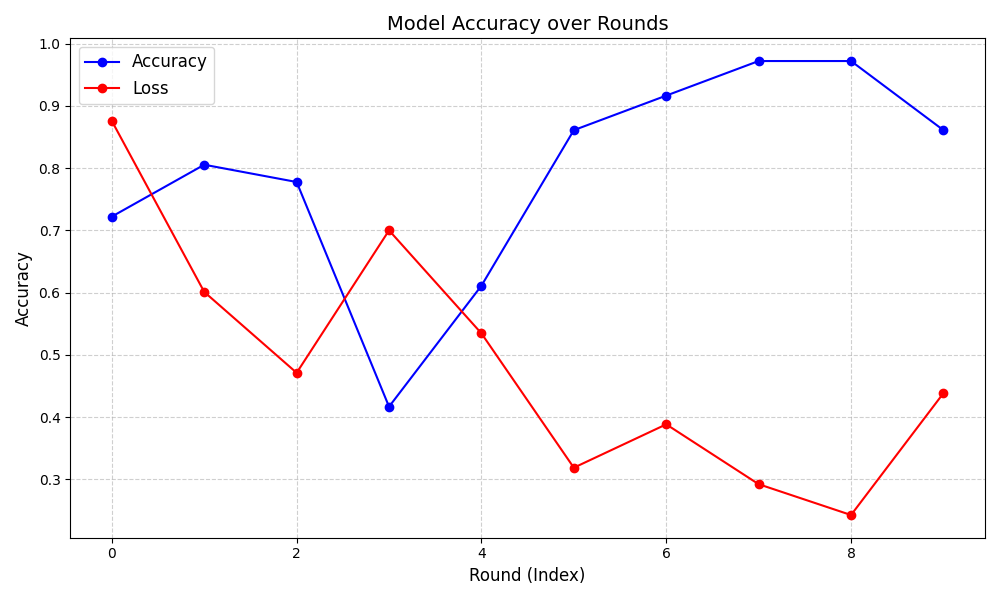
\includegraphics[width=0.8\textwidth]{figures/ml/honest-bfl.png}
  \caption{Federated Learning on a blockchain where nodes are all honest}
  \label{fig:honest-bfl}
\end{figure}

\begin{figure}
  \centering
  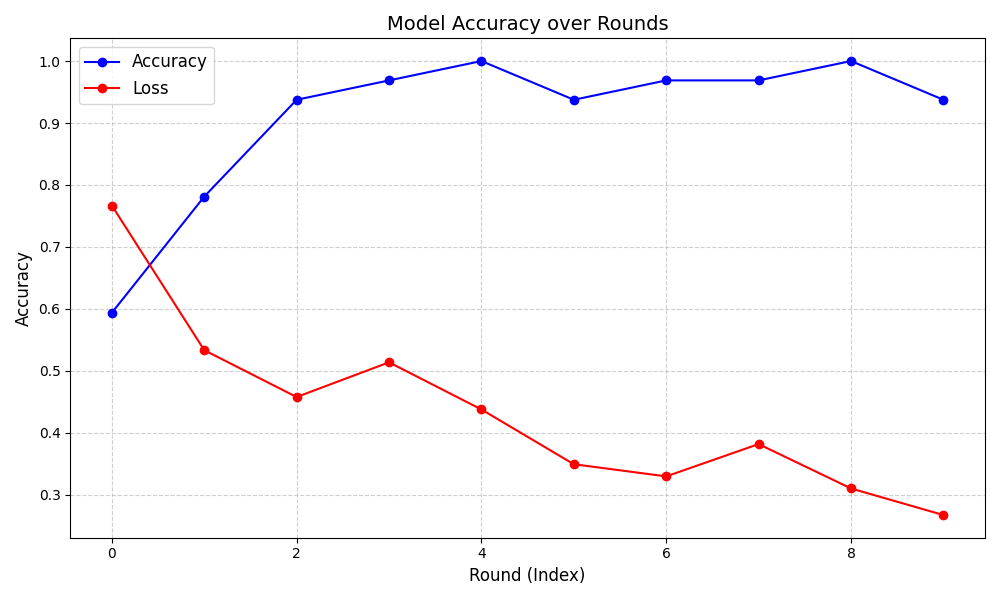
\includegraphics[width=0.8\textwidth]{figures/ml/honest-vfl.png}
  \caption{Vanilla Federated Learning where nodes are all honest}
  \label{fig:honest-vfl}
\end{figure}

\begin{figure}
  \centering
  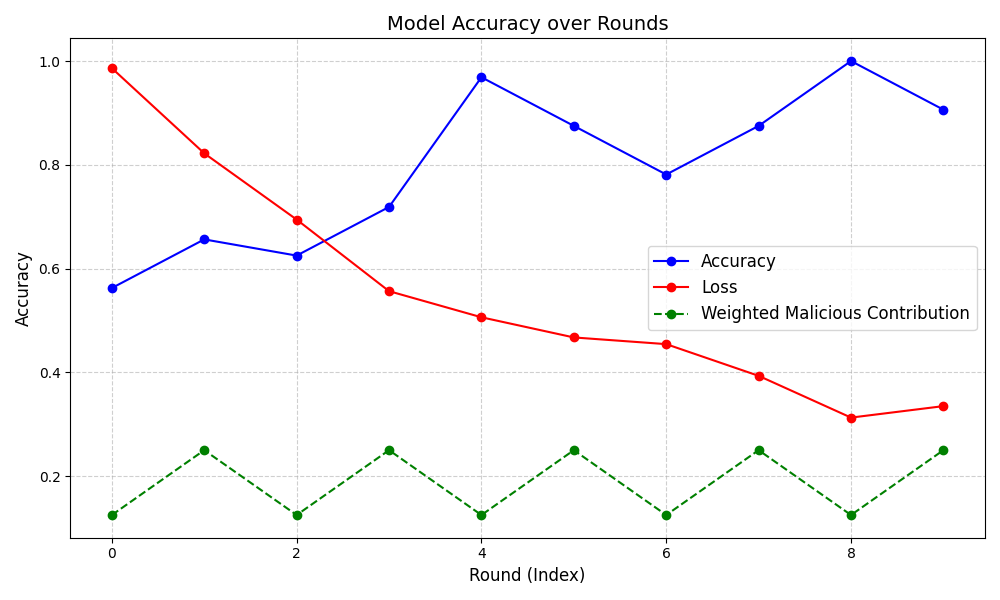
\includegraphics[width=0.8\textwidth]{figures/ml/malicious-bfl.png}
  \caption{Federated Learning on a blockchain where some nodes are malicious}
  \label{fig:malicious-bfl}
\end{figure}

\begin{figure}
  \centering
  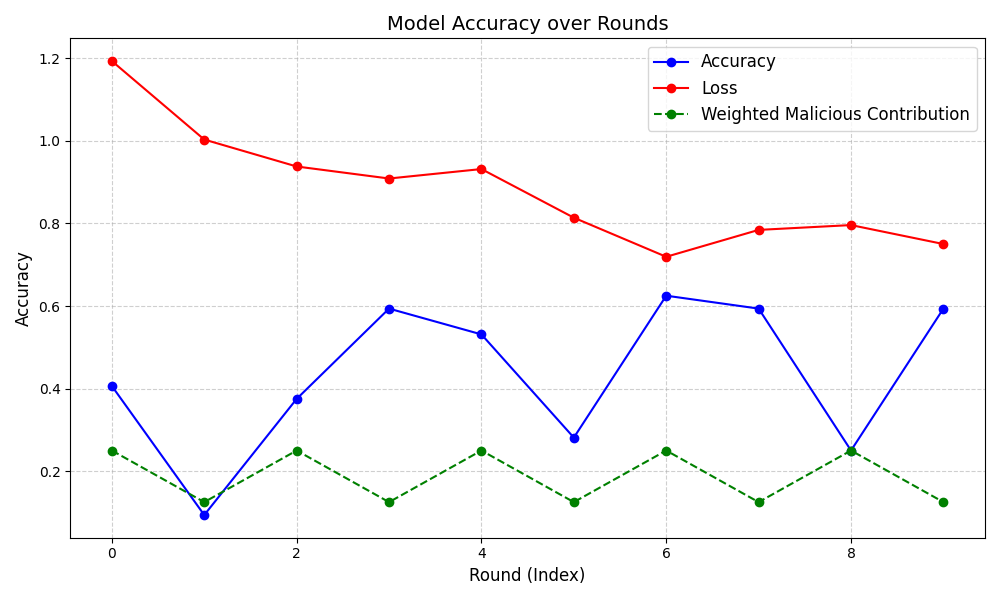
\includegraphics[width=0.8\textwidth]{figures/ml/malicious-vfl.png}
  \caption{Vanilla Federated Learning where some nodes are malicious}
  \label{fig:malicious-vfl}
\end{figure}
